% $Id: dev_guide.tex  $

\chapter{Developer's manual}
\minitoc

\section{Introduction}

As described in the Introduction, PRoNTo was developed using a modular structure. There are five main modules (`Data and Design', `Prepare Feature set', `Specify model', `Run model' and `Compute weights') and three reviewing and displaying modules (`Review data', `Review kernel and CV' and `Display results'). This structure not only facilitates the use of the toolbox but also new contributions from developers. These modules have very few dependencies between each other, and for most of them to work, one needs only to provide the `PRT.mat' obtained from the previous module and a few more module specific inputs. This means that the developer can contribute with code for any of the modules without having to adapt the whole toolbox to the changes.
\\

Developers can also work only on the module of interest and do not need to be familiar with the functions and sub functions that comprise the rest of the toolbox. In this chapter, we provide a brief description of how the code is organised and how one can contribute with new code, in particular new GUIs and Batch functions.
\\

After that, we provide instructions on how to integrate a new machine into PRoNTo. In the current version of PRoNTo, this is the most straightforward extension that can be added.
\\

And finally, we take an in-depth look into (1) the functions called at each step, (2) the PRT structure and its fields and (3) the files created at each step, as well as (4) the GUI and the batch behavior.


\section{Code organisation}

Although from the user's point of view there are five main modules, from the developer's side one can see PRoNTo's functions as belonging to three categories, depending on what they deal with (Figure \ref{Fig1.1}). The first set of functions and sub-functions is responsible for creating PRoNTo's GUIs and matlabbatch menu. The second set of functions comprise all the core routines that implement the machine learning methods (including extraction and preparation of the features, specification and estimation of a model, cross-validation, etc.). The last set of functions correspond to the actual machine learning algorithms that PRoNTo uses for classification and regression. We call these functions the `machines'. The main difference between this last set of functions and the rest, is that one does not need to be familiar with PRoNTo's PRT.mat structure or the rest of the code to be able to integrate a new machine. This can be done very easily, as shown below.

\begin{figure}[!htbp]
  \begin{center}
      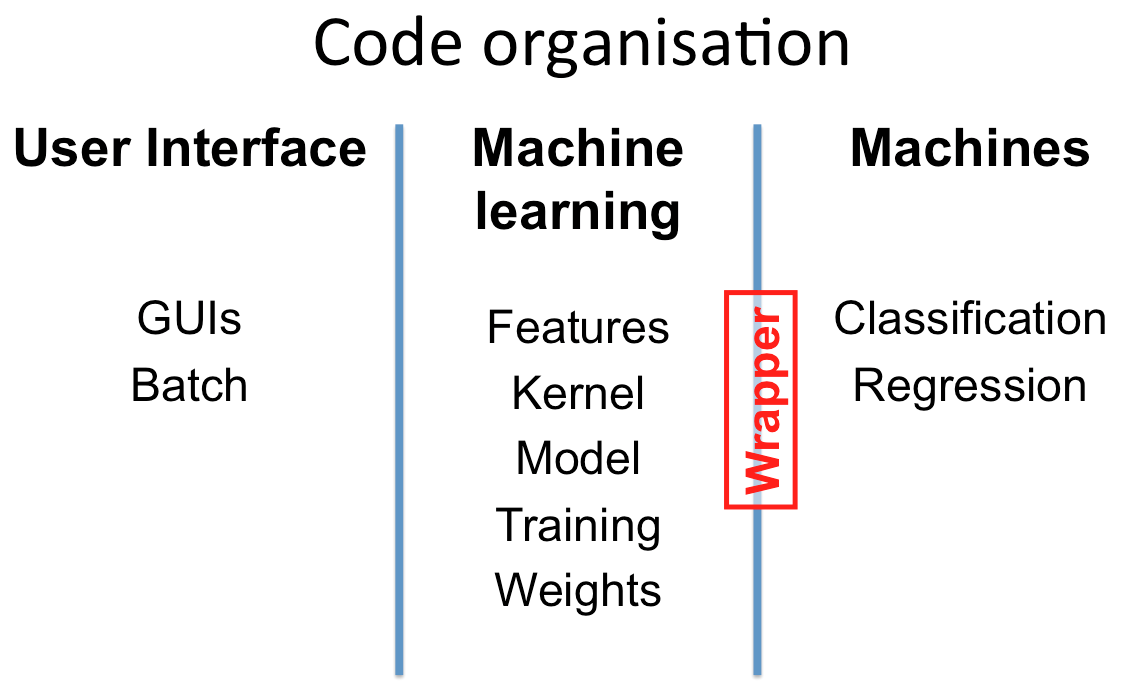
\includegraphics[height=2.2in]{images/code_pronto.png}
   \caption{Organisation of PRoNTo's functions. From the developer's perspective the code is organised in functions and sub functions that deal with the user interface experience (such as GUI and batch functions), the core functions that implement the machine learning approaches (including extracting and preparing the features, specification and estimation of a model, cross-validation routines, etc.) and the actual machine learning algorithms (also known as machines).}
    \label{Fig1.1}
  \end{center}
\end{figure}

\subsection{User interface}

The functions that deal with creating and running PRoNTo's main GUIs have the prefix `prt$\_$ui'. All GUI functions (`.m' files) have a corresponding `.fig' file. This file can be opened and edited using MATLAB's guide functionality. This way one can change the GUI and add extra options to the available menus (for more information, please consult MATLAB's documentation\footnote{http://www.mathworks.com/help/techdoc}).

PRoNTo's matlabbatch functions have either the prefix `prt$\_$cfg', to create a new menu on the batch interface and the prefix `prt$\_$run', to execute instructions using the variables from the corresponding `prt$\_$cfg' function. PRoNTo's batch functionalities work exactly like SPM. For more information on how to contribute with new matlabbatch functions please consult the developer's guide on the SPM8 manual\footnote{http://www.fil.ion.ucl.ac.uk/spm/doc/manual.pdf}.  

\subsection{Machine learning}

The machine learning routines comprise the core of PRoNTo. These routines do most of the necessary instructions to run all machine learning procedures currently implemented in the toolbox. They don't have a specific prefix but from the name of the .m file it is easy to find out what the function does (e.g. prt$\_$compute$\_$weights.m deals with creating new weights images). Most of the functions take as input the PRT.mat structure. Therefore, knowledge of this structure (see next chapter) is required in order to contribute with new code. In the future, we intend to make the process of introducing new feature selection algorithms and other model functionalities as easy as implementing a new machine, as described below.

\subsection{Machines}

Integrating a new machine algorithm, i.e. classifier or regressor, into the PRoNTo framework is straightforward. PRoNTo provides a function called `prt$\_$machine.m' that works as a wrapper around the different machine learning algorithms (functions with prefix `prt$\_$machine'). In brief, this wrapper translates PRoNTo's structure and internal variables into the required inputs for each machine. This way, the machine function needs only to read a simple input format that does not depend on knowledge of how PRoNTo works or of the PRT.mat fields (Figure \ref{Fig1.2}).

\begin{figure}[!htbp]
  \begin{center}
      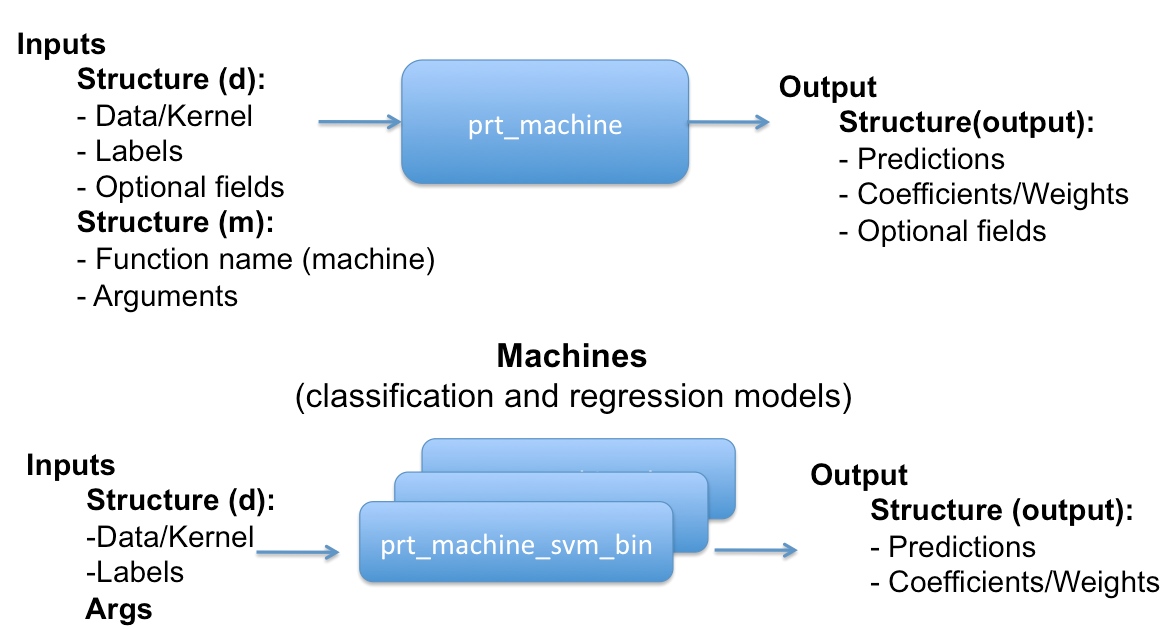
\includegraphics[height=3.0in]{images/machines.png}
   \caption{Code organisation for integrating a new machine with PRoNTo. `prt$\_$machine.m' works has a wrapper that translates PRoNTo's inputs into the machine format inputs and performs extensive error checks on these variables. The machines (such as `prt$\_$machine$\_$svm$\_$bin.m') perform the classifier/regression algorithms and have inputs and outputs that are not dependent on PRoNTo's internal structures.}
    \label{Fig1.2}
  \end{center}
\end{figure}

More specifically, to contribute with a new machine the developer needs to provide a matlab function, which reads the following input data structure, \textit{d}, and optional arguments, \textit{args}, (all fields are mandatory except where otherwise stated):

\begin{itemize}
\item \textit{d} - data structure with input to the classifier/regressor: \\
     \textit{.train} - training data (cell array of matrices of row vectors, each [Ntr x D]). Each matrix contains one representation of the data. This is useful for approaches such as multiple kernel learning. Ntr is the number of training examples and D is the dimension of the feature set (e.g. number of voxels).\\
     \textit{.test} - testing data  (cell array of matrices row vectors, each [Nte x D]). Nte is the number of testing examples and D the dimension of the feature set.\\
     \textit{.tr}$\_$targets - training labels (for classification) or values (for regression) (column vector, [Ntr x 1]).\\
     \textit{.use$\_$kernel} - flag: is data in form of kernel matrices (true) of in form of features (false)?
\item    \textit{args} (optional) - anything else that is specific to the algorithm (e.g. LIBSVM arguments).
\end{itemize}


\begin{figure}[!htbp]
  \begin{center}
      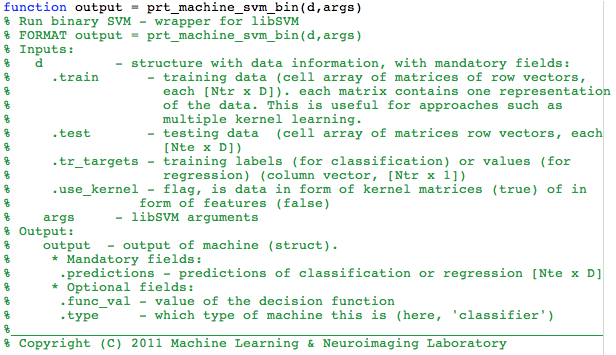
\includegraphics[height=3.0in]{images/prtmachinesvmbin.png}
   \caption{`prt$\_$machine$\_$.m' function help. Example of a PRoNTo machine for 2-class SVM classification.}
    \label{Fig1.3}
  \end{center}
\end{figure}

In addition, the outputs of the function need to have the following format, so that they can be read by the wrapper and translated back to the PRoNTo framework (all fields are mandatory except where otherwise stated) (Figure \ref{Fig1.2}):

\begin{itemize}
\item \textit{output}  - output structure with fields:\\
\textit{.predictions} - predictions of classification or regression [Nte x D]. Nte is the number of test examples and D the dimension of the feature set.\\
\textit{.func$\_$val} (optional) - value of the decision function (if it applies).\\
\textit{.type}  (optional) - type of machine (string: `classifier' or `regressor').
\end{itemize}

The rest of the function can be designed entirely as the developer wishes. The last thing to have in mind is the name of the function itself. It needs to have the prefix `prt$\_$machine' (e.g. `prt$\_$machine$\_$svm$\_$bin' is a function that implements support vector machine binary classification by calling the LIBSVM library). Importantly, the cross-validation and performance measures are performed outside in the main PRoNTo framework, and therefore the machine function should provide only the necessary instructions to implement the classifier/regressor algorithm.
\\

Finally, the new machine is easily integrated with PRoNTo by including the name of the file in the corresponding GUI and Batch functions (prt$\_$ui$\_$model.m and prt$\_$cfg$\_$model.m, respectively).
\\

The same procedure applies to the weights functions. PRoNTo provides a wrapper function called `prt$\_$weights'. The procedure for integrating a new weights function is exactly the same as for a new machine.
\\

Both wrapper functions, `prt$\_$machine' and  `prt$\_$weights', perform extensive tests to make sure the machines and weights code complies to the specific inputs and outputs required by the framework.
\\


\section{PRoNTo folder structure}

PRoNTo contains several subfolders. 

\begin{itemize}
\item The folder \_devUtils and \_unitTests are for testing. The folder atlas contains AAL atlas and its labels, and a Brodmann atlas without labels. If developers want to add atlases, this folder is the first choice.
 
\item The batch folders contains all files for the batch module, which includes both the configuration (with `cfg' in the function names) and job execution (with `run' in the function names) functions. For each step in PRoNTo, we have cfg and run batch files implemented. Configuration functions generates the trees defining the interfaces of the modules in Batch. Job execution functions pass user inputs to lower functions in PRoNTo for calculations and estimations. GUI and batch share the same lower functions for computations and estimations. This modular design eases the development of new machines and functions in each module. 

\item The machine folder contains the different regression and classification algorithms. There are functions from libraries, `machines' ( with `prt\_machine' in the function names) which interface the libraries to PRoNTo, and functions computing weights for each machine.  If developers want to add a machine, they can open these functions and read their inputs and outputs. Some naming conventions are: `gp' for Gaussian processes, `cla' for classification, `krr' for kernel ridge regression. Names of these algorithms also refer to libraries, for example, `gp' refers to the `gpml' library, `MKL' refers to the `simpleMKL' library. Details on these are in ref{XXXX}.

\item The manual folder contains latex files for the manual, images and other contents. Developers can add to the documentation here.

\item The masks folder contains one first-level mask in the Data \& Design module until before version 3. This changed in PRoNTo v3.0 and more masks (in nifti format) can be added.

\item In utils folder, there are several lower level functions e.g. checking if inputs are alpha numeric, or performing some operations on the kernels, such as split data in the kernel and normalise kernels. 
 
\item Beyond the above mentioned subfolders, functions with `ui' in their names define the GUI interfaces, i.e. *\_ui\_*.fig and *\_ui\_*.m file pairs define the figure and how the GUI behaves, respectively. We used GUIDE to create GUI and add custom functions and codes to extend these interface functions. 
 
\item The rest of the `prt\_' functions perform the computations and estimations defined in each module. 

\end{itemize}

%======================================================================



%======================================================================

\section{Data \& Design}

\subsection{PRT fields created}

PRT structure is created after specifying this module. More specifically, two fields of PRT.mat are filled: group and masks. Users input all their data, experimental design (e.g., modalities, runs, conditions) and other related information here (e.g. covariates, regression values). After this step, data information is stored in the group field of PRT.mat and nifti 1st level masks are stored in the masks field of PRT.mat.  HRF overlap and delay parameters are stored in masks field too. Below is a list of subfields in \textcolor{blue}{PRT.group} and \textcolor{blue}{PRT.masks}:

\begin{itemize}
\item \textcolor{blue}{PRT.group}

\begin{itemize}
\item \textcolor{blue}{PRT.group.gr\_name}: Storing group names
\item \textcolor{blue}{PRT.group.subject}: Storing subject information

\begin{itemize}
\item \textcolor{blue}{PRT.group.subject.subj\_name}: Storing subject names
\item \textcolor{blue}{PRT.group.subject.modality}: Subfields containing information on regression targets, covariates, modality name, design and scans. Note: classification labels are specified in Specify model module later.


\end{itemize}
\end{itemize}

\item \textcolor{blue}{PRT.masks}

\begin{itemize}
\item \textcolor{blue}{PRT.masks.mod\_name}: Name of corresponding modality
\item \textcolor{blue}{PRT.masks.type}: Type of the data
\item \textcolor{blue}{PRT.masks.fname}: The full path of the specified mask
\item \textcolor{blue}{PRT.masks.hrfoverlap}: Storing information on HRF overlap (default: 0)
\item \textcolor{blue}{PRT.masks.hrfdelay}: Storing information on HRF delay (default: 0)

\end{itemize}
\end{itemize}


%----------------------------------------------------------------------

\subsection{Files created}

PRT structure, saved in a PRT.mat file in the path specified by the user.


%----------------------------------------------------------------------

\subsection{GUI behaviour}

GUI of Data \& Design module provides interfaces for users to specify where to store the PRT structure and files, data information, experimental design, masks and all other related information.

\begin{itemize}
\item Save button creates PRT structure.
\item Load button loads previously created PRT.mat and checks its compatibility.
\item Review button provides a graphical review of all the input information and the interface for modifying some HRF parameters.
\end{itemize}
 
%----------------------------------------------------------------------

\subsection{Batch behaviour}

The Batch of Data \& Design module provides users similar functions and interfaces as GUI. However, there are some differences.

\begin{itemize}
    \item One is that the batch job can be saved as a .mat file or a .m function. Both users and developers can make changes directly in these files.
    \item Another difference is that both users and developers should be careful about the names of modalities when using the Batch. The names shall be consistent.
    \item One more difference is that HRF delay and overlap can be changed directly in the Batch of Data \& Design. In GUI, they can be modified in Review.
\end{itemize}

%----------------------------------------------------------------------

\subsection{Functions called}


\textbf{\underline{GUI:}}

\begin{enumerate}

\item \textcolor{red}{prt\_ui\_design.m} and \textcolor{red}{prt\_ui\_design.fig}

The functions define GUI interfaces and the figure for Data \& Design module. It initializes the code, executes each button press in this module in GUI, checks if the inputs are correct and creates output in MATLAB prompt. If developers want to make changes in this GUI module (e.g., a button’s or menu’s functions), you’ll find subfunctions with corresponding names in \textcolor{red}{prt\_ui\_design.m} and add codes there. % are sub-functions with illustrations pointing you which code segments define which button press.
Some important functions called by \textcolor{red}{prt\_ui\_design.m} are summarized as follows.

% Sub-functions include:
\begin{itemize}
\item \textcolor{red}{prt\_data\_modality.m} and \textcolor{red}{prt\_data\_modality.fig}

The two files define the GUI panel for specifying the information of the modality, experimental design, covariates and regression targets. The \textcolor{red}{prt\_data\_modality.m}  also calls:

\begin{itemize}
\item \textcolor{red}{prt\_data\_conditions.m} and \textcolor{red}{prt\_data\_conditions.fig}, for receiving inputs for conditions, i.e. experimental design.
\item \textcolor{red}{prt\_check\_design.m}, for checking the design and discards scans according to overlapping conditions or the minimum time interval between conditions based on the HRF function and specified HRF parameters.
\end{itemize}

\item \textcolor{red}{prt\_get\_defaults.m} and \textcolor{red}{prt\_defaults.m}

Default settings of PRoNTo are stored in \textcolor{red}{prt\_defaults.m}, including global defaults such as colour, parameters for the data and design, preprocessing, default atlas for ROI definition, arguments of different machines, and parallelization of the code. The function \textcolor{red}{prt\_get\_defaults.m} gets the relevant default values from \textcolor{red}{prt\_defaults.m} for this module. For instance, the code `color=\textcolor{red}{prt\_get\_defaults}(`color')' sets colors of backgrounds and figure parameters for Data \& Design module.

\item \textcolor{red}{prt\_data\_review.m} and \textcolor{red}{prt\_data\_review.fig}

The two functions define the GUI for reviewing the data.

\end{itemize}

\item \textcolor{red}{prt\_load.m} and \textcolor{red}{prt\_struct.m}

This function is called by \textcolor{red}{prt\_ui\_design.m}. When clicking the load button, the functions are called to load PRT.mat and check the fields in it for backwards compatibility. If you add a field somewhere in the PRT and that field is necessary for display or further analyses, the prt\_struct file should be amended to set default values for that field to ensure that older PRT files can still be read and modified.

\end{enumerate}

\noindent \textbf{\underline{Batch:}}

\begin{enumerate}
    \setcounter{enumi}{2}

\item \textcolor{red}{prt\_cfg\_design.m} and \textcolor{red}{prt\_run\_design.m}

\begin{itemize}
\item Function \textcolor{red}{prt\_cfg\_design.m} is the Data \& Design module configuration file and builds the PRT.mat data and design structure.
\item Function \textcolor{red}{prt\_run\_design.m} is the job execution function, which takes a harvested job data, rearranges them into PRT structure and saves it.
\end{itemize}

\end{enumerate}

At this stage, the GUI and batch have very little code in common. Hence, changes in the GUI have to be performed independently in the batch and conversely.  


%======================================================================



%======================================================================

\section{Prepare feature set}

\subsection{PRT fields created}

There are two fields created in PRT.mat in this step, too. Field \textit{fs} (feature set) and \textit{fas} (file array structure). The information for the two fields is specified by users in the `Specify modality to include' panel.

For each modality, a file array is created containing the data (detrended if specified) from the selected modality. The field \textcolor{blue}{PRT.fas} is linked to this file array. In \textit{fas}, the information stored refers to the modality (as defined in Data \& Design). This means that multiple MRI sessions, entered as different runs will each create a \textit{fas}. A \textit{fas} links to a \textit{.dat} file with dimensions of \#images x \#features within the first-level mask and stores feature operations (detrend and detrend parameters), header of the first image for recovering images if needed, and indices of all features within the first-level mask.
\\

The field \textit{fs} refers to the kernel/feature set that is created. It is a structure of size number of feature sets created by the user. Within \textit{fs}, there is information on feature set name, kernel file, ID matrix, information of using multiple kernels. This field also contains information about the second-level mask and/or the atlas (used to build the kernel).
\\

One important subfield is the ID matrix, which contains information about the modalities selected in the feature set arranged in six different columns: group, subject, modality, condition, block and scan.

\begin{itemize}
\item The name of the columns are stored in \textcolor{blue}{PRT.fs.id\_col\_names}.
\item The group numbers, subject numbers, modality labels, condition numbers, block labels and scan numbers themselves are stored in \textcolor{blue}{PRT.fs.id\_mat}, whose dimension is the number of samples x 6.
\end{itemize}

The ID matrix is referred to in the `Review kernel \& CV' reviewing tool in PRoNTo, where a graphical display shows the structure of this matrix.

\begin{itemize}
\item In addition, there is a \textit{fas} subfield in \textcolor{blue}{PRT.fs}, that is different from \textcolor{blue}{PRT.fas}. This subfield in \textit{fs} refers to the modality and scan indices of the feature set modalities in the \textit{fas} structure. It is useful when modalities are concatenated in samples (e.g. accessing the correct scans from multiple runs in an MRI experiment, with each run linked to a different \textcolor{blue}{PRT.fas} file array).

\end{itemize} 

% \begin{itemize}
% \item \textcolor{blue}{PRT.fs}

% \begin{itemize}
% \item \textcolor{blue}{PRT.fs.fs\_name} - 
% \item \textcolor{blue}{PRT.fs.k\_file} - 
% \item \textcolor{blue}{PRT.fs.id\_col\_name} - 
% \item \textcolor{blue}{PRT.fs.} - 
% \item \textcolor{blue}{PRT.fs} - 
% \item \textcolor{blue}{PRT.fs} - 
% \item \textcolor{blue}{PRT.fs} - 


% \end{itemize}

% \item \textcolor{blue}{PRT.masks}

% \end{itemize}


%----------------------------------------------------------------------

\subsection{Files created}

\begin{itemize}
\item FAS .dat file.
\item A kernel matrix (.mat with variable Phi, a cell array with a kernel in each cell).
\item Updated masks and/or atlases (nifti resampled at the size of the input data images).
\end{itemize}


%----------------------------------------------------------------------

\subsection{GUI behaviour}

The GUI of `Prepare feature set' takes the PRT.mat created in Data \& Design module and provides interfaces for users to further specify feature sets, their names, selected modalities, operations on feature sets and the atlas for defining kernels. 


%----------------------------------------------------------------------

\subsection{Batch behaviour}

The module of `Prepare feature set' in the Batch is similar to the GUI. However, the batch requires consistent names across modules. Running important modules altogether will overwrite the PRT.mat, hence delete the links between the PRT.mat and the computed feature set(s) and kernel(s). \textit{FAS} will be recreated each time the Batch is launched. More detailed illustrations on this please refer to \ref{sec:matlabbatch_3_4}.


%----------------------------------------------------------------------

\subsection{Functions called}

\textbf{\underline{Core:}}

\begin{enumerate}

\item \textcolor{red}{prt\_fs.m}

Gather information on the modalities to build file arrays containing the (detrended) data and computes the linear kernels. It resizes the second-level masks and atlas if needed. \textcolor{red}{prt\_fs.m} calls:
\begin{itemize}
\item \textcolor{red}{prt\_init\_fs.m} to populate basic fields in \textcolor{blue}{prt.fs}, like the file array structure, kernel data structure and feature set parameters. 
\item \textcolor{red}{prt\_fs\_modality.m} to write the kernel matrix to the user-defined path as well as the feature set if needed.
\end{itemize}

\item \textcolor{red}{prt\_init\_fs.m}

     This function initialises the next function (\textcolor{red}{prt\_fs\_modality.m})
     
\item \textcolor{red}{prt\_fs\_modality.m}

    For each selected modality, builds and reads from the file array to compute the kernel. It calls \textcolor{red}{prt\_get\_defaults.m} to get defaults about fs, and \textcolor{red}{prt\_load\_blocks.m} to access one or more blocks of data to avoid memory overload. 

\end{enumerate}


\noindent \textbf{\underline{GUI:}}

\begin{enumerate}
\setcounter{enumi}{3}

\item \textcolor{red}{prt\_ui\_prepare\_data.fig} and \textcolor{red}{prt\_ui\_prepare\_data.m}

GUI to specify how many feature sets will be used in the feature set. In v2, these modalities can either be concatenated (e.g. multiple runs of an experiment), or used in multiple kernel settings (e.g. sMRI grey and white matter). For each modality entered, the function calls \textcolor{red}{prt\_ui\_prepare\_datamod.m} to specify parameters for this specific modality.

\begin{itemize}
\item \textcolor{red}{prt\_ui\_prepare\_datamod.fig} and \textcolor{red}{prt\_ui\_prepare\_datamod.m}

Functions \textcolor{red}{prt\_ui\_prepare\_datamod.m} and \textcolor{red}{prt\_ui\_prepare\_datamod.fig} are called by \textcolor{red}{prt\_ui\_prepare\_data.m} to accept user inputs about modalities, to compute the file array and for building the kernel.
\end{itemize}

\end{enumerate}

\noindent \textbf{\underline{Batch:}}

\begin{enumerate}
\setcounter{enumi}{4}

\item \textcolor{red}{prt\_cfg\_fs.m} and \textcolor{red}{prt\_run\_fs.m}

The fs configuration file constructs the feature set for each modality. The related job execution function harvests all inputs passed by \textcolor{red}{prt\_cfg\_fs.m} and arrange them into the PRoNTo structure. It calls \textcolor{red}{prt\_fs.m} to build file arrays and compute kernels from them.


\end{enumerate}




%======================================================================



%======================================================================

\section{Specify model}

Specify model module computes the inputs for the models, but does not estimate/run the models. Main inputs for this module are feature sets, where users select which feature set will be used to build the model, model type (regression or classification), selection of samples and classes, machines, cross validation (CV) strategy and data operations.

\subsection{PRT fields created}

Two subfields in \textcolor{blue}{PRT.model} are created and filled: \textcolor{blue}{PRT.model.model\_name}, which stores the name of the model and \textcolor{blue}{PRT.model.input} which stores all the other information. Another subfield \textcolor{blue}{PRT.model.output} is only created but is not filled here. It will be filled after the model is estimated (Run model module). Below is an illustration of the information stored in \textcolor{blue}{PRT.model.input}:
 
\begin{itemize}
 
\item \textcolor{blue}{PRT.model.input.use\_kernel}: 1 (use kernel methods). From version 3 there is also option 0 (non-kernel methods).

\item \textcolor{blue}{PRT.model.input.type}: Regression or classification. This field is being visited very often within PRoNTo.

\item \textcolor{blue}{PRT.model.input.machine}: Stores information of the chosen machine. The algorithms can be found in the subfolder \textit{PRoNTo/machines/}.

\item \textcolor{blue}{PRT.model.input.use\_nested\_cv}: Whether to optimize hyperparameters (1) or not (0).

\item \textcolor{blue}{PRT.model.input.nested\_param}: A vector of user-defined parameters if \textcolor{blue}{PRT.model.input.use\_nested\_cv} is 1. This can also be empty, which means to leave it for the algorithm to set values by default. The default values are specified in \textcolor{blue}{PRT\_nested\_CV} at the `Run model' step.

\item \textcolor{blue}{PRT.model.input.cv\_type\_nested}: The CV strategy for the inner CV loop.

\item \textcolor{blue}{PRT.model.input.cv\_k\_nested}: Value of k for the k-fold inner CV loop. If 10 is here, it means that the strategy takes 90\% of the data for training, and 10\% of the data for test.
\begin{itemize}
\item Leave-one-out has k=0.
\end{itemize}

\item \textcolor{blue}{PRT.model.input.subsample}: 

\item \textcolor{blue}{PRT.model.input.indmodels}:

\item \textcolor{blue}{PRT.model.input.class}: Contains the user-specified selection for each class. 

\begin{itemize}
\item It's a structure of size number of classes (classification) or 1 (regression). It specifies the groups, subjects within that group and conditions for each class, with a similar structure as in \textcolor{blue}{PRT.group} (without the modalities). And we identify which indices in the global ID matrix are selected to build the specified class.
\item The CV matrix and everything else are built from here. This can be viewed in Review kernel \& CV. Note: it’s always good to have a check on the CV matrix to ensure the inputs do what you want. You can also make a CV matrix yourself and input via Custom choice in Cross-validation scheme. In the Review module, you can view the classes specified.
\end{itemize}


\item \textcolor{blue}{PRT.model.input.samp\_idx}: Index of the selected samples for this model, in the corresponding feature set.

\item \textcolor{blue}{PRT.model.input.include\_allscans}:


\item \textcolor{blue}{PRT.model.input.targets}: Prediction targets for building the model.

\item \textcolor{blue}{PRT.model.input.targ\_allscans}:

\item \textcolor{blue}{PRT.model.input.covar}:

\item \textcolor{blue}{PRT.model.input.cov\_allscans}:

\item \textcolor{blue}{PRT.model.input.cv\_k}: Value of k for the k-fold outer CV loop (i.e. the main or external CV).

\item \textcolor{blue}{PRT.model.input.cv\_mat}: CV matrix for the external CV.

\item \textcolor{blue}{PRT.model.input.cv\_type}: CV type for the external CV.

\item \textcolor{blue}{PRT.model.input.operations}: Stores user selected data/kernel operations as an integer vector. The operations will be applied according to this order. 
 
\end{itemize} 

Specify model module creates and estimates inputs for estimating the model. It is easy to script. For example, higher-level users and developers can copy \textcolor{blue}{PRT.model} and change any of the sub-fields listed above when it is needed manually. CV matrix is computed based on CV schemes specified by the user.

%----------------------------------------------------------------------

\subsection{Files created}

No new files are created at this stage.


%----------------------------------------------------------------------

\subsection{GUI behaviour}

In GUI, users can choose Specify model alone or Specify and run model. It computes the sample indices based on the classes, computes CV matrix based on the ID matrix (and labels in case of `Leave-per-Group-Out') and CV specifications, and it gathers the targets and covariates based on the class definition. ID matrix is used here as a reference to obtain these sub-groups of indices, targets and covariates for building the particular model. CV matrix can also be input by users via Custom CV.


%----------------------------------------------------------------------

\subsection{Batch behaviour}

Batch provides similar functions to GUI, but the Specify model and Run model modules are separated.

%----------------------------------------------------------------------

\subsection{Functions called}

\textbf{\underline{Core:}}

\begin{enumerate}

\item \textcolor{red}{prt\_model.m}

This function initialises the model data structure (by calling \textcolor{red}{prt\_init\_model.m}), computes targets and the sample index.

\begin{itemize}
\item In PRoNTo v2.1, classification and regression are addressed differently. In classification, the codes visit information stored in the design. For regression, only subject-level analysis is available, so the codes do not go into the design.
The sub-functions compute\_targets and compute\_target\_reg inside \textcolor{red}{prt\_model.m} compute the prediction targets for classification and regression, respectively. Targets that are not selected for this model are put to zeros. From PRoNTo v3.0 both classification and regression compute the prediction targets using an updated version of the compute\_targets sub-function.
\end{itemize}
 
\item One note is that the labels of different classes are 1,2,3,..., here referring to Class 1, Class 2, Class 3, ... respectively. They will be converted to class labels accepted by the actual machines inside the machine function, if needed. For example, if Faces and Houses are selected by the user as Class 1 and Class 2, respectively, and if we use SVM, the labels 1 and 2 will be converted to -1 and 1 in the machine \textcolor{red}{prt\_machine\_svm\_bin.m}.

\item \textcolor{red}{prt\_compute\_cv\_mat.m}

It computes the CV matrix. Inner and external CV loops call the same function. This function is accessed in the Specify model and Run model modules. In PRoNTo, CV schemes are shown in abbreviations, for example:

\begin{itemize}
\item LOSO: leave-one-subject-out. If we have 56 subjects, and 10 folds. Then 5 subjects in each fold, the remaining 6 will be distributed to the first 6 folds. As a result, 6 subjects in the 1 to 6 folds, 5 subjects in the remaining 4 folds. The reason to do this is for distributing subjects more evenly.
\item LORO:leave-one-run-out. There is no leave-multiple-run-out option in PRoNTo, only leave-one-run-out.
\end{itemize}

Other CV schemes can be found in the user manual. PRoNTo also provides interfaces for users to input their own CV design, i.e. the custom CV. Users can input their own CV matrix via this interface. The codes for this part here only check things. Relevant codes of the interface do the real work. Please note that nested CV  will not be computed in Specify model step, but during the model estimation.
 
\end{enumerate}


\noindent \textbf{\underline{GUI:}}



\begin{enumerate}
\setcounter{enumi}{2}

\item \textcolor{red}{prt\_ui\_model.m}  and \textcolor{red}{prt\_ui\_model.fig}

The GUI functions that define the interfaces of Specify model module. It calls several other functions among which:

\begin{itemize}
\item \textcolor{red}{prt\_ui\_select\_class.m} and \textcolor{red}{prt\_ui\_select\_class.fig}

This function provide interfaces to users to select classes for classification problems.


\item \textcolor{red}{prt\_ui\_select\_reg.m} and \textcolor{red}{prt\_ui\_select\_reg.fig}

This function provide interfaces to users to select data for regression analysis in regression problems.

\item \textcolor{red}{prt\_ui\_specify\_CV\_basis.m} and \textcolor{red}{prt\_ui\_specify\_CV\_basis.fig}

This function provides interfaces for users to input their custom CV information. It calls \textcolor{red}{prt\_ui\_custom\_CV.m} and \textcolor{red}{prt\_ui\_custom\_CV.fig} to allow custom CV specification.

\item \textcolor{red}{prt\_model.m}

This function configures and builds the \textcolor{blue}{prt.model} structure.

\item \textcolor{red}{prt\_cv\_model.m}

This function runs a CV on a given model.

\end{itemize}


\end{enumerate}


\noindent \textbf{\underline{Batch:}}


\begin{enumerate}
\setcounter{enumi}{6}

\item \textcolor{red}{prt\_cfg\_model.m} and \textcolor{red}{prt\_run\_model.m}

Functions define the tree and behaviors of the Specify model module in the Batch.


\end{enumerate}




%======================================================================



%======================================================================

\section{Run model}

Specify model sets up the configuration of the model. Run model module performs the training and testing. It includes hyperparameter optimization by using inner cross-validation (CV) schemes, model training and testing using external CV schemes, computing statistics for model performance measures and PRT.mat updates. The machine is called in this module for model evaluation. In GUI, this module can be run directly from Specify model. In Batch, it is separated from the Specify module.
\\

\noindent \textbf{\underline{How is the cross-validation implemented?}}
\\

CV schemes are important to model training and testing. In PRoNTo, this is mainly performed by \textcolor{red}{prt\_cv\_model.m}. After some initialization steps, it begins the main CV loops, i.e. external CV loops. If the user chooses to optimize hyperparameters, each fold from the external CV is sent to inner CV schemes. Users can choose different CV strategies for inner and external CV. The function \textcolor{red}{prt\_nested\_cv.m} is called to optimize hyperparameters. The best hyperparameter is returned to \textcolor{red}{prt\_cv\_model.m} within each external fold. Whether hyperparameter is optimized or not, one model is estimated per fold by calling \textcolor{red}{prt\_cv\_fold.m}. This is followed by statistic computations for model performance measures, by calling \textcolor{red}{prt\_stats.m}. In \textcolor{red}{prt\_cv\_model.m}, statistics are calculated and stored at fold level and model level. Model level statistical metrics are obtained by concatenating results across folds in version 2. This changed to averaging metrics across folds in version 3. PRT.mat is updated and saved in the end of \textcolor{red}{prt\_cv\_model.m}.
\\[2cm]

\noindent \textbf{\underline{How is the parameter optimization implemented?}}
\\

In many situations, it is preferable to optimize hyperparameters to increase the predictive model performance. If users choose this step, each external fold is sent to \textcolor{red}{prt\_nested\_cv.m} and goes through an inner CV loop. The training data in this external fold is splitted into training and testing sets inside \textcolor{red}{prt\_nested\_cv.m} according to the inner CV schemes. Before looping over inner CV folds, \textcolor{red}{prt\_nested\_cv.m} checks user-defined hyperpameter ranges. Default ranges are used if there are no user inputs. Hence, this function first loops over each hyperparameters and then loops over inner folds for each hyperparameter. It calls \textcolor{red}{prt\_cv\_fold.m} to perform the model training and testing. One model is created for each inner fold, generating predictions. Within every loop of a certain hyperparameter, model performance metrics are calculated for each inner fold.
\\

Statistic calculation is done by calling \textcolor{red}{prt\_stats.m}. In version 2, we concatenate predictions from each inner fold to obtain the model-level performance measures. Specifically, balanced accuracy is used for classification and MSE is used for regression. This generates one metric value per hyperparameter. After completing the inner CV for all values of the hyperparameter, we choose the best one according to the metrics, i.e. the hyperparameter generating the maximum balanced accuracy is selected as the best one for classification and the hyperparameter generating the minimum MSE is selected as the best one for regression. \textcolor{red}{prt\_nested\_cv.m} returns the best hyperparameter to \textcolor{red}{prt\_cv\_model.m} for the outer model training and testing.
\\

\noindent \textbf{\underline{How are the machines organized?}}
\\

Model training and testing for both external and inner CV are done by calling \textcolor{red}{prt\_cv\_fold.m}. This function configures model parameters and applies user-specified data operations before feeding them to the machines. It calls \textcolor{red}{prt\_machine.m} which will then distribute to the specific machine A structure containing data information related to CV folds and information of the selected machine are passed to \textcolor{red}{prt\_machine.m}. After some input checks, \textcolor{red}{prt\_machine.m} passes these information to the specific machine function. The machine-specific functions are in the machine folder, with ‘machine’ in their names. Some of them are wrapper functions of the core functions in several third-party libraries, such as Libsvm, Liblinear and SimpleMKL.
\\

PRoNTo uses wrapper functions to organise inputs (data, class labels, targets, function arguments and hyperparameters) to formats accepted by actual machines in those libraries, and organise outputs from these machines to PRoNTo accepted formats. For instance, \textcolor{red}{prt\_machine\_svm\_bin.m} is a wrapper of binary SVM in Libsvm. PRoNTo takes the hyperparameter range from GUI or Batch, then combines it with other machine arguments required by Libsvm. Training and testing datasets are organised according to Libsvm conventions. Predictions and model parameters from the binary SVM machine are stored according to PRoNTo conventions. Machine arguments include options provided by third-party libraries and hyperparameters (e.g. C for SVM). Most of the type, we define machine options in \textcolor{red}{prt\_defaults.m}.
\\
 
\noindent \textbf{\underline{What are the input and output for a machine?}}
\\

Generally speaking, each \textcolor{red}{prt\_machine\_*.m} function accepts two inputs, a structure d containing the data information and a structure args containing machine-specific information including options and hyperparameter values. In structure d: d.train and d.test contain the training and testing data respectively. The d.tr\_targets refers to targets of the training data. There is no need to pass d.te\_targets as model performance is evaluated outside of the machine, in PRoNTo \textcolor{red}{prt\_stats.m}. One flag d.use\_kernel contains information about whether the machine is a kernel machine or not.. In version 2, this is by default always true. The output of each machine contains prediction values, function values from the decision function, model parameters and the type of the machine (classifier or regression). 
% \\[2cm]


%----------------------------------------------------------------------


\subsection{PRT fields created}

Two new fields are created in PRT.mat in this module: \textcolor{blue}{PRT.model.output.fold}, \textcolor{blue}{PRT.model.output.stats}. In \textcolor{blue}{PRT.model.output.fold}, several subfields are generated to store information of hyperparameter effects, prediction values in each fold, fold-level statistics, decision function values, model parameters and other information specific to some machines (e.g. kernel contributions for MKL models).

%----------------------------------------------------------------------

\subsection{Functions called}

\textbf{\underline{Core:}}

\begin{enumerate}

\item \textcolor{red}{prt\_cv\_model.m}, \textcolor{red}{prt\_nested\_cv.m} and \textcolor{red}{prt\_cv\_fold.m}

This function is where CV schemes are implemented within PRoNTo. Before looping over CV folds, it gets the model index, configure variables based on the CV matrix, gets values and variables for model estimation, such as user-specified targets, class numbers, kernels, and machine arguments. It also initializes outputs. This function calls \textcolor{red}{prt\_nested\_cv.m} to optimize hyperparameters. It calls \textcolor{red}{prt\_cv\_fold.m} to train and test the predictive models. \textcolor{red}{prt\_nested\_cv.m} also calls \textcolor{red}{prt\_cv\_fold.m} within each inner fold to estimate models. 
       
\item \textcolor{red}{prt\_stats.m}

This function is called by \textcolor{red}{prt\_cv\_model.m} to calculate fold-level and model-level metrics measuring the model performance. It takes predictions, model type, test targets, and class numbers as inputs.  For classification, confusion matrix, accuracy, balanced accuracy, class accuracy and predictive value are calculated.  For regression, MSE (and normalized MSE), correlation and squared correlation are calculated. These metric values are passed as outputs in a `stats' structure.
       
\item \textcolor{red}{prt\_machine.m} and \textcolor{red}{prt\_machine\_*.m} functions

These functions are in the machine folder carrying out the actual modeling. \textcolor{red}{prt\_machine.m} is called by \textcolor{red}{prt\_cv\_fold.m} and passes data information and machine arguments to the machine-specific functions \textcolor{red}{prt\_machine\_*.m}, which are generally wrapper functions of the core machines provided by several third-party libraries. These wrapper functions perform some initial checks on the inputs, re-structure data and arguments to formats accepted by the core machines, then checks outputs from the estimated models and organize them into PRoNTo accepted structures. 

\end{enumerate}


\noindent \textbf{\underline{GUI:}}

\begin{enumerate}
\setcounter{enumi}{3}

\item \textcolor{red}{prt\_ui\_model.m} calls \textcolor{red}{prt\_cv\_model.m} to start Run model module if the user clicks `Specify and Run'.

\item \textcolor{red}{prt\_ui\_cv\_model.m} and \textcolor{red}{prt\_ui\_cv\_model.fig}

These are functions implementing the GUI interface for Run model. It loads the specified models from the PRT and fills a list that the user can select from. \textcolor{red}{prt\_cv\_model.m} is called sequentially on the models selected for estimation.

\end{enumerate}

\noindent \textbf{\underline{Batch:}}

\begin{enumerate}
\setcounter{enumi}{5}

\item \textcolor{red}{prt\_cfg\_cv\_model.m} and \textcolor{red}{prt\_run\_cv\_model.m}

These are the batch functions defining the trees of the Run Model module and execute the configurations. It accepts inputs from \textcolor{red}{prt\_cfg\_model.m}, organise them into proper structures. From version 2 and on, permutation test is interfaced in Batch in this module.

\end{enumerate}


%======================================================================



%======================================================================

\section{Compute weights}


Two steps are used to compute weights, that are carried out by prt\_compute\_weights.m and prt\_weights\_*.m for specific machines. Weight maps can be built as voxel-wise images or ROI-wise images. For multiple kernel learning, maps indicating kernel contributions with ranking information can be obtained.
\\

\noindent \underline{\textbf{How are the weights computed in PRoNTo?}}
\\
 
The function \textcolor{red}{prt\_compute\_weights.m} accepts information from \textcolor{red}{PRT.m} and some user-defined information, such as which model the weight image is for, where to save, flags indicating whether to build weights for each permutation (batch only) and/or for each ROI, and atlas for ROI-wise weight image if it is selected by the users. If different modalities were used without concatenating the samples, one weight map is built for each modality.
\\
 
For each modality, weight computation is classified into classification and regression problems. One weight image will be built per class for multi-class problems, while only one weight map is built for binary classification or regression problems. These are implemented in \textcolor{red}{prt\_compute\_weights\_class.m} and \textcolor{red}{prt\_compute\_weights\_regre.m}, respectively. Processing routines for classification and regression are similar to each other. Take classification as an example to illustrate the routine. The code finds the type of data (nifti or MEEG) and machine first, then creates image names. One tricky part is the multiple indexing step. Getting the correct indices from the file array (.dat file), feature sets and each slice along z axis within ROIs is implemented here. In Prepare feature set module, we need a subset of images to build the file array, from which we use potentially a subset to build a kernel. In order to build the weight image, we therefore need to access indices from both file arrays and feature sets fs structures. To not to overload the memory, we build the weight image slice by slice along the z axis, since most images are 3-D files. So we need to take indices from that slice, within both the second-level and the first-level masks. The three levels of indices are necessary to build weight maps.
\\
 
The next step is to create maps. If the user selects to build weight images for each permutation, relevant checks and codes are in \textcolor{red}{prt\_compute\_weights.class.m}. Image initialization is performed before the weight computation. During weight computation, we access indices within the 2nd level mask along the z axis. For weight maps using the whole brain, we use similar approaches with slightly different inputs. In \textcolor{red}{prt\_compute\_weights.m}, the variable flag2 tells if we want to get one weight per region instead of one weight per voxel, so weight computation will be changed according to this. We build one image for each fold, which results in a 4-D image where the last map is an average over all folds. Data operations are applied. If MKL is used, codes get Beta here. Following procedures are to build the weights, reshape them into the correct dimensions, normalize the weights for visualization and save the images.
\\
 
The code performing actual multiplication for weights is done by using \textcolor{red}{prt\_weights.m} in the machine folder within \textcolor{red}{prt\_compute\_weights\_class.m} and \textcolor{red}{prt\_compute\_weights\_regre.m}. This function calls other \textcolor{red}{prt\_weights\_*.m} in the machine folder. Since different machines have different formulations, computing weights using outputs from these machines may vary too. Take \textcolor{red}{prt\_weights\_sMKL\_cla.m} as an example: the inputs are structure d and args similar to inputs to machines. But the data loaded in \textcolor{red}{prt\_compute\_weights\_class.m} and \textcolor{red}{prt\_compute\_weights\_regre.m} is d.datamat. By taking coefficients from d.coeffs and data from d.datamat, multiplications for weight values are carried out in these \textcolor{red}{prt\_weights\_*.m} functions.


%----------------------------------------------------------------------

\subsection{Files created}

This module creates image files of weights. Weight maps have ‘weights\_*’ and/or ’ROI\_weights\_*‘ in their names. Maps of ROIs are separated from voxel-wise maps which can be identified by names. In PRT.mat, extra fields are created:

\begin{itemize}
\item \textcolor{blue}{PRT.model.output.weight\_img}, \textcolor{blue}{PRT.model.output\_weight\_ROI} if building weights for ROIs is selected and subfields saving information of rankings of weights.

\item \textcolor{blue}{prt.model.output\_weight\_MOD} if weights for MKL are selected.

\end{itemize}

Display weights functionality searches for \textcolor{blue}{PRT.model.output.weight\_img} to locate where the maps are.


%----------------------------------------------------------------------


\subsection{Functions called}

% \textbf{\underline{Core:}}

\begin{enumerate}

\item \textcolor{red}{prt\_compute\_weights.m}, \textcolor{red}{prt\_compute\_weights\_class.m}, and \textcolor{red}{prt\_compute\_weights\_regre.m}
 
PRoNTo calls \textcolor{red}{prt\_compute\_weights.m} to implement weight image computation. This function accepts several inputs: PRT.mat, user defined inputs including model name, image name, path to save the maps, atlas and two flags. It outputs image files with specific names. This function finds the right model, loops over feature sets and saves PRT.mat. Within feature set loops, it computes the number of images according to whether it is a classification problem (class numbers) or regression problem. It then starts loops over file arrays, where building weights for classification and regression is done by calling functions \textcolor{red}{prt\_compute\_weights\_class.m}, and \textcolor{red}{prt\_compute\_weights\_regre.m}, respectively. Computing weights for each voxel for a whole brain and for ROIs are processed differently. Different processings for MKL and for multiple kernels but only one modality are implemented.
\\
 
Routines within  \textcolor{red}{prt\_compute\_weights\_class.m}, and \textcolor{red}{prt\_compute\_weights\_regre.m} are very similar. One part requires some attentions is the multi-level indexing step. The two functions also call \textcolor{red}{prt\_weights.m} and \textcolor{red}{prt\_weights\_*.m} to perform the actual multiplications for weight computations. They build weight maps per fold and a map as an average across folds, then save images.    
 
\item \textcolor{red}{prt\_weights}, \textcolor{red}{prt\_weights\_bin\_linkernel.m}, and \textcolor{red}{prt\_weights\_*.m} for other machines

These functions are in the machine folder. Formulations of different machine may vary, so weight computations may be machine-specific. We get coefficients from the kernel space, then map them back to the original space. When adding new machines, corresponding weight computations shall be considered and added too. There are some general cases in PRoNTo, where \textcolor{red}{prt\_weights\_bin\_linkernel.m} can be used. Other \textcolor{red}{prt\_weights\_*.m} functions implement multiplications for machines beyond the linear kernel case.
\\
 
One example of the machine-specific weight function is \textcolor{red}{prt\_weights\_sMKL\_cla.m}. It accepts input structures d and args, creates weight vector as the output. In structure d:

\begin{itemize}
\item d.datamat: the data being loaded in \textcolor{red}{prt\_compute\_weights\_class.m} and \textcolor{red}{prt\_compute\_weights\_regre.m}.
\item d.coeffs:– coefficients, such as alphas generated by using SVM.
\item d.betas: this is the kernel contributions, specific to sMKL.
\item d.idfeat\_img: voxel indices of the features in the image.
\end{itemize}

\end{enumerate}



%======================================================================



%======================================================================

\section{Results}

During Run Model module, predictions, decision function values, weights and metrics measuring the model performance are computed. These results are stored in several subfields in \textcolor{blue}{PRT.output}.
\\

\noindent \underline{\textbf{How are the performance metrics computed?}}
\\

Within each main CV fold, statistics are computed at fold level. After looping over all folds, we concatenate predictions from each fold and pass them to \textcolor{red}{prt\_stats.m} together with true targets to compute model-level statistics. Formulations and codes calculating these metrics are in \textcolor{red}{prt\_stats.m}. ROC and AUC for binary classification are calculated in Display results module by calling \textcolor{red}{prt\_plot\_ROC.m} in version 2. This is moved to \textcolor{red}{prt\_stats.m} in version 3.


%----------------------------------------------------------------------

\subsection{Functions called}

% \textbf{\underline{Core:}}

\begin{enumerate}

\item \textcolor{red}{prt\_stats.m}

The same as described in Compute weights module. 

\item \textcolor{red}{prt\_plot\_ROC.m}

This function takes PRT, model index, fold and graphical information as inputs, then obtains true positive and false positive rates to build ROC curves and calculates AUC. This is done for each fold. Averaged results over folds are given too.  

\end{enumerate}

















